\documentclass[11pt]{article}
\usepackage[utf8]{inputenc}
\usepackage[margin=2.3cm]{geometry}
\usepackage{indentfirst}
\usepackage{tikz}
\usepackage{multicol}
\usepackage{graphicx}
\usepackage{wrapfig}
\usepackage{blindtext}
\usepackage{amsmath}
\usepackage{adjustbox}
\usepackage[version=4]{mhchem}
\usepackage{graphicx}
\usepackage{caption}
\usepackage{float}
\usepackage[section]{placeins}
\usepackage{adjustbox}
\usepackage{setspace}
\usepackage{listings}
\usepackage{subcaption}
\usepackage{hyperref}
\definecolor{capt}{RGB}{12,12,12}

\setstretch{1.2}

\captionsetup{
  format = hang,
  font = footnotesize,
  labelfont = {bf},
}

\setlength{\parskip}{5pt}
\setlength\parindent{0pt}

\addtolength{\jot}{1em}

\lstdefinestyle{myStyle}{
    belowcaptionskip=1\baselineskip,
    breaklines=true,
    frame=none,
    basicstyle=\small,
    backgroundcolor=\color{gray!7},
}

% \lstset{framexleftmargin=5mm, frame=shadowbox, rulesepcolor=\color{blue}}


\title{\textbf{Experiment: Numerical solution of the time-independent 1-D Schr{\"o}dinger equation}}
\author{Dominik Kuczynski (student id: 21367544)}
\date{Sep-Oct 2023, Monday AM}

\begin{document}

\maketitle

\tableofcontents

\newpage

\section{Abstract}

For arbitrary potential, the Schr{\"o}dinger equation quickly becomes
impossible to solve analytically. 

Here, energy eigenstates of the infinite well and bounded harmonic 
potential were found using a "shooting" method
together with a numerical integration scheme. The found values
correspond well (to within 5\%) with the analytic solution.

The uncertainties of $x$ and $p$ in both potentials were calculated
at different energy states and the uncertainty principle was shown
to hold.

Finally, the bounded harmonic potential energies were shown to be
approximately evenly spaced for the first 10 states, and become
quadratic - as in the case of the infinite well - past that point.

% include all results!

\section{Overview}

The Schr{\"o}dinger equation is one of the most important equations
of quantum mechanics. It can be, however, extremely difficult or
even impossible to solve analytically for different potentials. 
For that reason, numerical methods utilizing discretization are
commonly used to integrate solutions for a given energy. Finding the
values of energy which produce physical wavefunctions - an eigenvalue
problem - is a challenge in itself. One approach to solving it is
to utilise some properties of the equation to recursively approach
these values up to some given tolerance.

\subsection{Analytical solutions}

In considering a system contained within a finite region of space, say from
$x=0$ to $x=L$, and with a given potential and particle mass, the
Schr{\"o}dinger equation in dimensionless form is:
\begin{align}
     &\frac{d^2 \psi(\tilde{x})}{d\tilde{x}^2}+\gamma^2 (\epsilon-\nu(\tilde{x})))\psi(\tilde{x})=0
     \label{eq:2}
\end{align}

where$\qquad\tilde{x}=x/L,\quad \epsilon=E/V_0,\quad \nu(\tilde{x})=V(\tilde{x})/V_0,\quad \gamma^2=\frac{2mL^2V_0}{\hbar^2}$.

To solve Equation \ref{eq:2} for the infinite potential well, write:
$  \nu(\tilde{x})=
  \begin{cases}
    -1,\quad 0<\tilde{x}<1\\
    \infty,\quad \text{else.}
  \end{cases}$

In the allowed ($0<\tilde{x}<1$) region, Equation \ref{eq:2} has
a simple solution of the form:
$$\psi(\tilde{x})=c_1 e^{i \gamma \sqrt{\epsilon+1} x} +c_2 e^{-i \gamma \sqrt{\epsilon+1} x}$$

The disallowed region imposes additional conditions that $\psi(\tilde{x})=0$
for $\tilde{x}\leq0$ or $\tilde{x}\geq1$. These as well as normalisation
allow for the solving of $c_1$ and
$c_2$, as well as restrict the values of $\omega$. The final solution becomes:
\begin{equation}
  \psi(\tilde{x})=\sqrt{2}\sin(\gamma \sqrt{\epsilon+1} \tilde{x}),\quad \gamma\sqrt{\epsilon+1}=2\pi n
\end{equation}
\begin{equation}
  \implies \epsilon_n=\frac{4\pi^2n^2}{\gamma^2}-1,\quad n=1,2,...
  \label{eq:epsilon}
\end{equation}
Note in particular, the energy values increase quadratically with $n$.

To solve for the harmonic potential, first consider the dimensionful solution when
$V(x)=\frac{1}{2}k x^2$\cite{grif}:
\begin{equation}
  E_n=(n+\frac{1}{2})\hbar \omega,
  \quad \psi_n(x)=\left(\frac{m\omega}{\pi \hbar}\right)^{1/4}\frac{1}{\sqrt{2^n n!}}H_n(\xi)e^{-\xi^2/2},
  \quad n=0,1,2,...
\end{equation}

To convert the potential into the dimensionless form being analysed,
$\nu(\tilde{x})=8(\tilde{x}-0.5)^2-1$,\\
 set $k=  \frac{16V_0}{L^2}$.  This allows us to solve for $\epsilon_n$:
\begin{equation}
  \epsilon_n=E_n/V_0=(n+\frac{1}{2})\frac{\hbar}{V_0}\sqrt{\frac{k}{m}}-1=
  (n+\frac{1}{2})\frac{4\sqrt{2}}{\gamma}-1
\end{equation}

Note that here $E$ was shifted down by $V_0$, together with $V(x)$.
Here the energy values are evenly spaced.

To calculate $\Delta \tilde{x}=\sqrt{\langle \tilde{x}^2\rangle-\langle\tilde{x}\rangle^2}$,
it is useful to note that for symmetric potentials, the particle is as likely to be 
"on the left" as it is "on the right" of the axis of symmetry, meaning $\langle \tilde{x}\rangle$
is precisely the position of that axis. In the cases examined here, $\langle x \rangle=0.5$.

The second moment of $\tilde{x}$ can be calculated using
\begin{equation}
  \langle\tilde{x}^2\rangle=\int_0^1 \tilde{x}^2|\psi(\tilde{x})|^2d\tilde{x}
\end{equation}

To find the uncertainty $\Delta \tilde{p}$, one needs to use that the 
non-dimensional momentum operator is $\hat{\tilde{p}}=-i\frac{d}{dx}$.
Then, $\langle \tilde{p}\rangle=\langle\psi^*|\hat{\tilde{p}}|\psi\rangle$=
$-i\int_0^1\psi\frac{d\psi}{d\tilde{x}}d\tilde{x}$ for real $\psi$. But since
$\psi(0)=\psi(1)=0$, integration by parts of the above yields that
$\langle\hat{\tilde{p}}\rangle=0$.

Similarly, $\langle \tilde{p}^2\rangle=\langle\psi^*|\hat{\tilde{p}}^2|\psi\rangle$=
$-\int_0^1\psi\frac{d^2\psi}{d\tilde{x}^2}d\tilde{x}$ and therefore:
\begin{equation}
  \Delta\tilde{p}=\sqrt{-\int_0^1\psi\frac{d^2\psi}{d\tilde{x}^2}d\tilde{x}}.
\end{equation}

\section{Method}

To solve the Schr{\"o}dinger equation numerically, the variable $\tilde{x}$ gets
discretized into $N$ values\\
 $x_n\ ,\ n=1,2,...,N$, between 0 and 1. Then, 
the value of $\psi$ at a given point $x_{n+1}$ can be approximated using the
values of $\psi$ and $\nu$ at two previous points:

\begin{equation} 
  \label{eq:4}
  \psi_{n+1}\approx\frac{2(1-\frac{5}{12}l^2k_n^2)\psi_n-(1+\frac{1}{12}l^2k^2_{n-1})\psi_{n-1}}{1+\frac{1}{12}l^2k^2_{n+1}}
  \qquad\text{with }k_n^2=\gamma^2(\epsilon-\nu(\tilde{x}_n))
\end{equation}

This allows for the numerical integration of $\psi(\tilde{x})$ from 0 to 1,
 given its values at the two
initial points $x_1$ and $x_2$.
To obtain $\psi$'s second derivative at a given point, the finite difference
scheme was used. Denoting by $l$ the separation of discrete points $x_n$:
\begin{equation}
  \psi_n''\approx\frac{\psi_{n-1}-2\psi_n+\psi_{n+1}}{l^2}
\end{equation}

When the value $\epsilon$ is given, a numerical integration algorithm, following
(\ref{eq:4}) can 
generate a wavefunction, provided two initial conditions.
For the purposes of this lab, the conditions were the following:
$\psi(x_1)=0,\quad \psi(x_2)=10^{-4}$.

\subsection{Shooting method for finding energy eigenstates}

Since the energy spectrum of the infinite well potential is discrete, only specific
values of energy will produce normalizable (physical) wavefunctions. 
The method used for finding these values makes use of the fact that non-eigenstate
energies will produce wavefunctions blowing up to positive or negative
values at the end of the interval.
However, since the final result is continuous in $\epsilon$, 
between two energies producing $\psi$ blowing
up with opposite signs, there must be one for which $\psi(1)=0$.

\begin{lstlisting}[language=Python, style=myStyle]
  def shoot(energy, v, tol=5e-4, de=5e-3):
      # initialize e to a starting value
      e = energy

      # variable for storing psi(1) of the previous iteration
      prevLastPsi = 0

      while(abs(de) > tol):
          psi = integratePsi(e, v)
          psi = normalize(psi)
          # if the sign of psi(1) has changed, move to in between 
          # the last two energies
          if psi[-1] * prevLastPsi < 0:
              de = -de/2

          prevLastPsi = psi[-1]
          e += de

      return e
\end{lstlisting}

\section{Results \& Discussion}
\vspace{-.4cm}
\subsection{Infinite well potential}

The wavefunctions of the first three found eigenstates were plotted and
the result appears to correspond to the analytic solutions. To actually
check the accuracy, the error in the first eigenstate was plotted and found to
be less than 0.005.

\begin{figure}[htbp]
  \begin{minipage}{.5\textwidth}
    \centering
    \includegraphics*[width=0.851\linewidth]{ex_eigenstates1.png}
    \captionsetup{width=0.9\textwidth}
    \vspace{-.3cm}
    \caption{First three generated eigenstates of the infinite well potential}
  \end{minipage}%
  \begin{minipage}{0.5\textwidth}
    \centering
    \includegraphics*[width=0.85\linewidth]{error_sin.png}
    \captionsetup{width=0.9\textwidth}
    \vspace{-.3cm}
    \caption{Absolute error between the generated and analytic solution}
  \end{minipage}
\end{figure}

\begin{table}[h]
  \centering
  \caption{Normalised eigenstate energies $\epsilon_n$ - infinite well}
  \label{tab:1}
  \vspace{-.3cm}
  \begin{tabular}{c|c|c|c}
    n & numerical result (\texttt{tol=1e-5}) & analytic result & absolute error\\
    \hline
    1 & -0.95055 & -0.95065 & $0.00010$\\
    2 & -0.80220 & -0.80260 & $0.00040$\\
    3 & -0.55498 & -0.55586 & $0.00088$\\
    4 & -0.20884 & -0.21043 & $0.00159$\\
    5 &  0.23616 &  0.23370 & $0.00247$\\
    6 &  0.78008 &  0.77652 & $0.00355$\\
    7 &  1.42290 &  1.41805 & $0.00485$\\
    8 &  2.16459 &  2.15827 & $0.00632$\\
    9 &  3.00518 &  2.99718 & $0.00800$\\
    10 &  3.94469 &  3.93480 & $0.00989$

  \end{tabular}
\end{table}

The obtained eigenstate energies were compared with the analytical
results for a given tolerance and the errors were calculated
(Table \ref{tab:1}).

\begin{wrapfigure}[9]{r}{0.5\textwidth}
  \vspace{-1cm}
  \centering
  \captionsetup{width=0.4\textwidth}
  \includegraphics*[width=0.4\textwidth]{error_vs_tol.png}
  \vspace{-.3cm}
  \caption{Absolute error in eigenstate energies vs. tolerance}
\end{wrapfigure}

To further investigate how the tolerance 
value affects the accuracy, the errors of the first three energies were
plotted for different tolerances.
It is clear that the tolerance value affects the resulting accuracy significantly.
However, the above figure also shows the existence of other sources of error - 
which have the dominant effect when tolerance is low enough.

\vspace{.4cm}
It seems most likely that the main source of these errors would be the accuracy of
the numerical integration. This is consistent with the observed relation where 
higher energies, corresponding to more rapidly oscillating and thus more error-prone
wavefunctions, have larger errors.

The uncertainty relation for the infinite well potential was checked by plotting 
$\Delta x \Delta p$ at the calculated eigenstate energies $\epsilon_n$.
It is clear that the uncertainty increases with energy, and the minimum
value of $1/2$ is never achieved.

\begin{figure}[h]
  \centering
  \includegraphics*[width=0.6\textwidth]{uncertainty1.png}
  \caption{Uncertainty relation - infinite well}
\end{figure}

\subsection{Bounded harmonic potential}

\begin{table}[htbp]
  \centering
  \caption{Normalised eigenstate energies $\epsilon_n$ - bounded harmonic potential}
  \vspace{-.3cm}
  \begin{tabular}{c|c|c|c}
    n & numerical result (\texttt{tol=1e-9}) & analytic result & absolute error\\
    \hline
    0 &-0.910557280&-0.910557281 & 0.000000001\\
    1 &-0.731671835&-0.731671843 & 0.000000008\\
    2 &-0.552786242&-0.552786405 & 0.000000163\\
    3 &-0.373898901&-0.373900966 & 0.000002065\\
    4 &-0.194996989&-0.195015528 & 0.000018539\\
    5 &-0.016005948&-0.016130090 & 0.000124141\\
    6 & 0.163395485& 0.162755348 & 0.000640137\\
    7 & 0.344230419& 0.341640786 & 0.002589633\\
    8 & 0.528873026& 0.520526225 & 0.008346801\\
    9 & 0.721278843& 0.699411663 & 0.021867180
  \end{tabular}
  \label{tab:2}
\end{table}

The calculated eigenstate energies were, again, compared to the analytical solutions.
However, since there is no analytic solution for the harmonic potential bounded by
infinite walls, the solutions of the unbounded harmonic potential was used to compare.
The discussion of this approximation can be found in the later part of this section.

Again, like in the case of the infinite well, it is clear that there are other
sources of error than the set tolerance - particularly at higher energies.

This time, in plotting the uncertainty,
20 of the first eigenstate energies were used. Again, as in the 
previous case, the uncertainty increases linearly with energy,
however this time reaching the minimum value of $1/2$ at $n=0$.

\begin{figure}[!h]
    \centering
    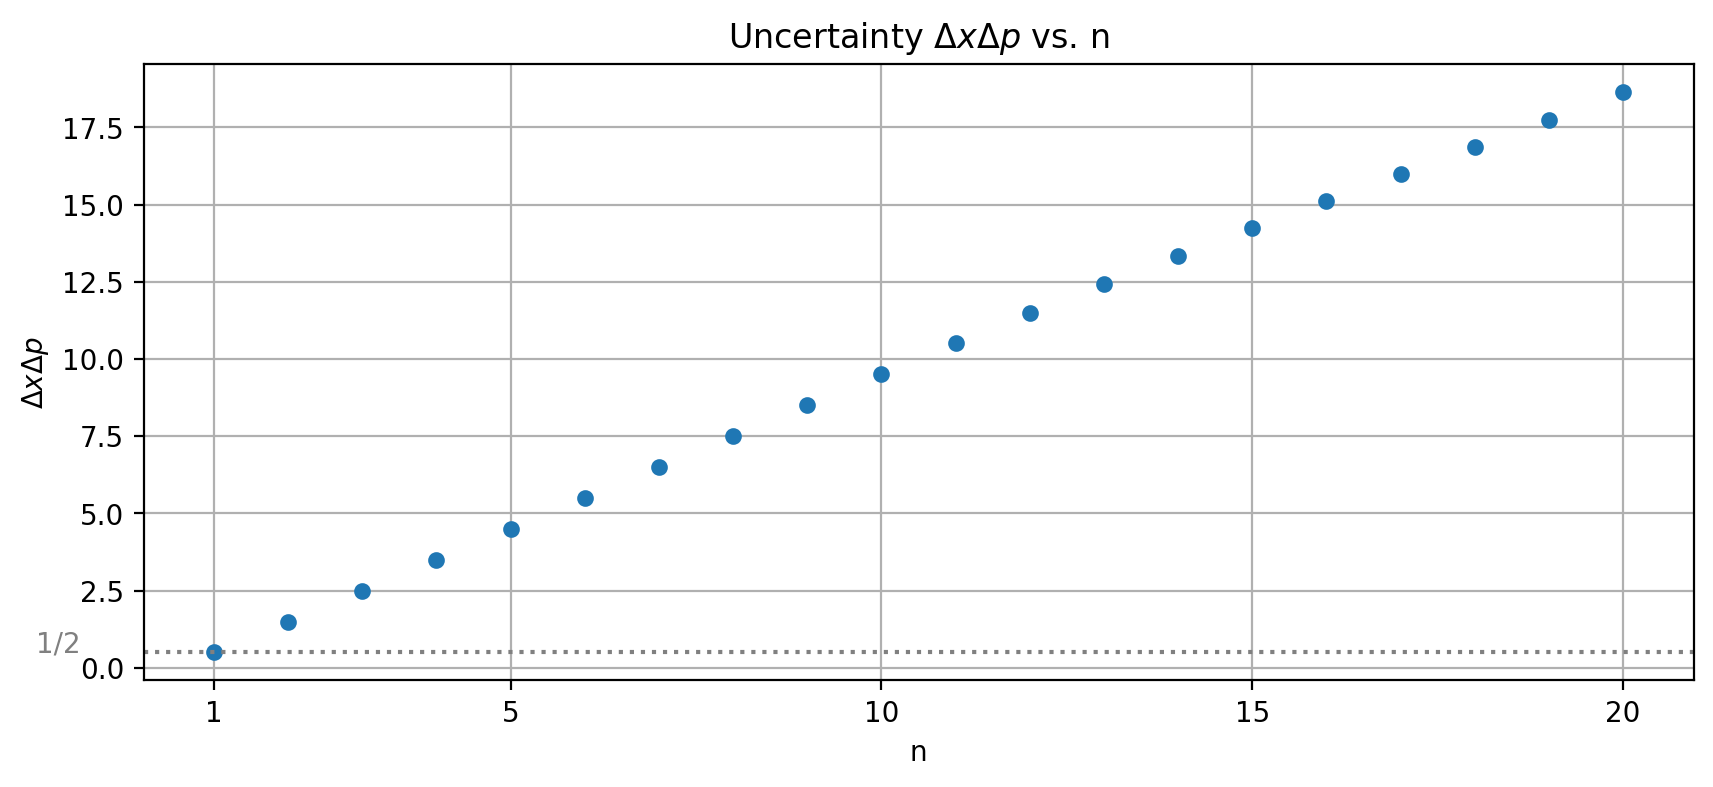
\includegraphics[width=0.65\textwidth]{uncertainty2.png}
    \caption{Uncertainty relation - bounded harmonic potential}
\end{figure}

\pagebreak

\begin{figure}[!h]
  \begin{subfigure}{0.5\textwidth}
    \centering
    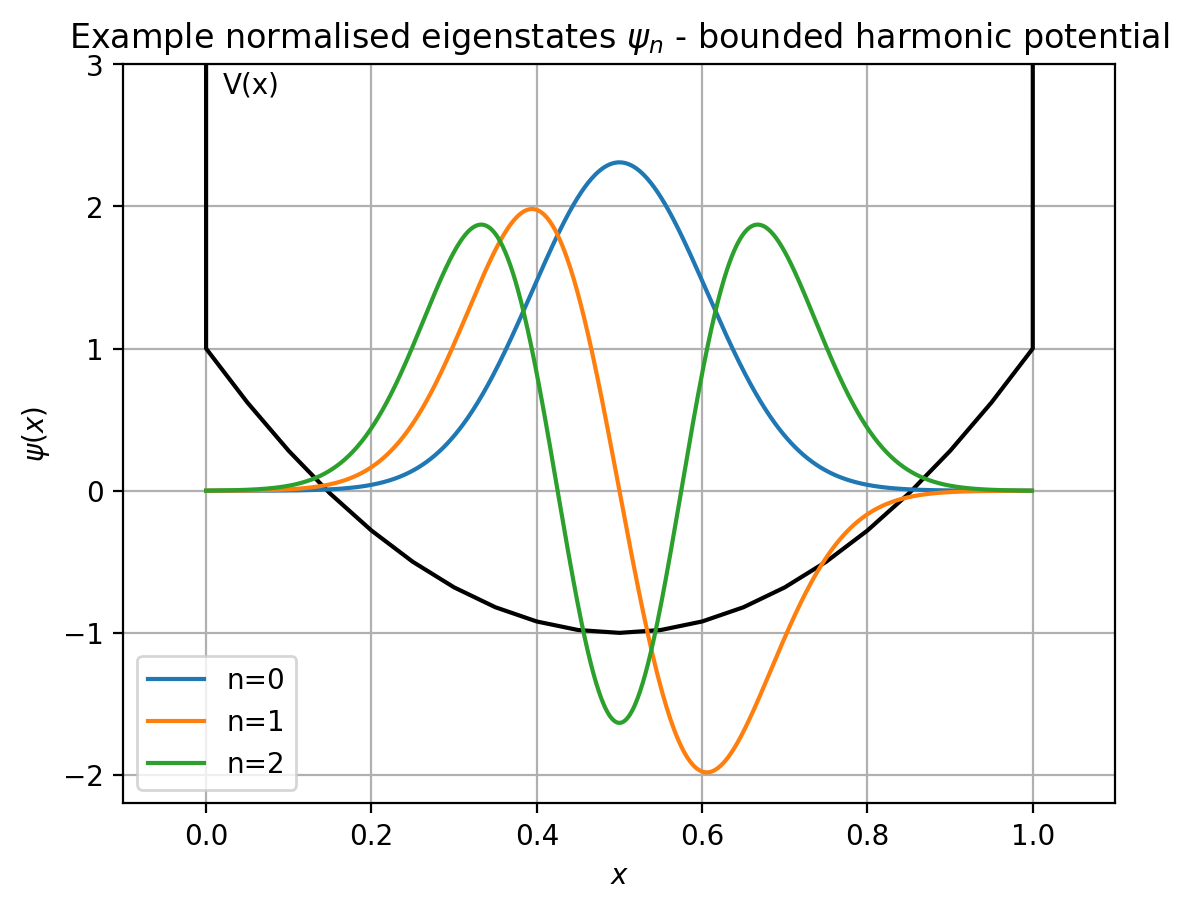
\includegraphics[width=\linewidth]{ex_eigenstates2.png}
    \caption{Low energy states}
  \end{subfigure}%
  \begin{subfigure}{0.5\textwidth}
    \centering
    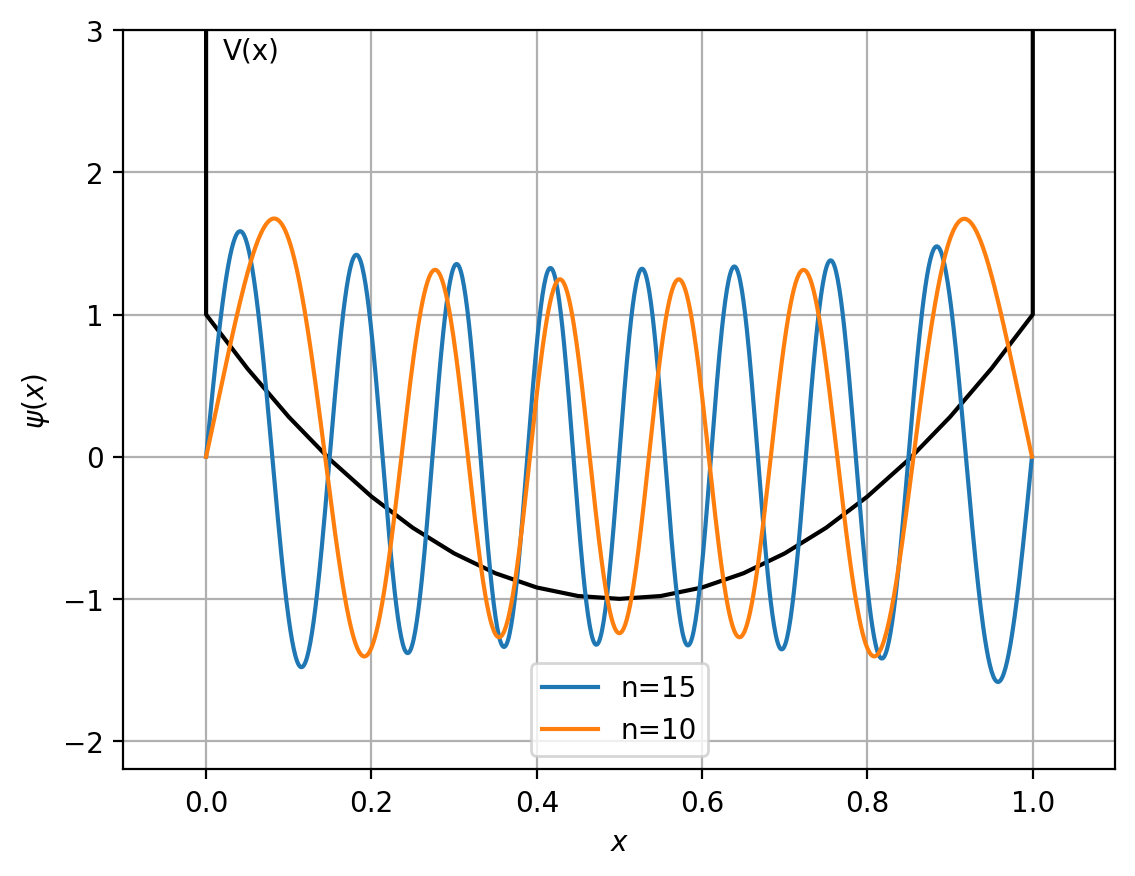
\includegraphics[width=\linewidth]{ex_eigenstates3.png}
    \caption{High energy states}
  \end{subfigure}
  \caption{Example eigenstates of the bounded harmonic potential}
\end{figure}

The above plots of the generated eigenstates show that the bounded
harmonic approximation is accurate at lower energies but breaks down
at higher ones.
There, the system effectively starts behaving like an infinite
square well - 
the solutions appear to have roots at $x=0$ and $x=1$, instead of identically 
converging to 0.

\begin{wrapfigure}[8]{R}{0.5\textwidth}
  \vspace{-1.1cm}
  \centering
  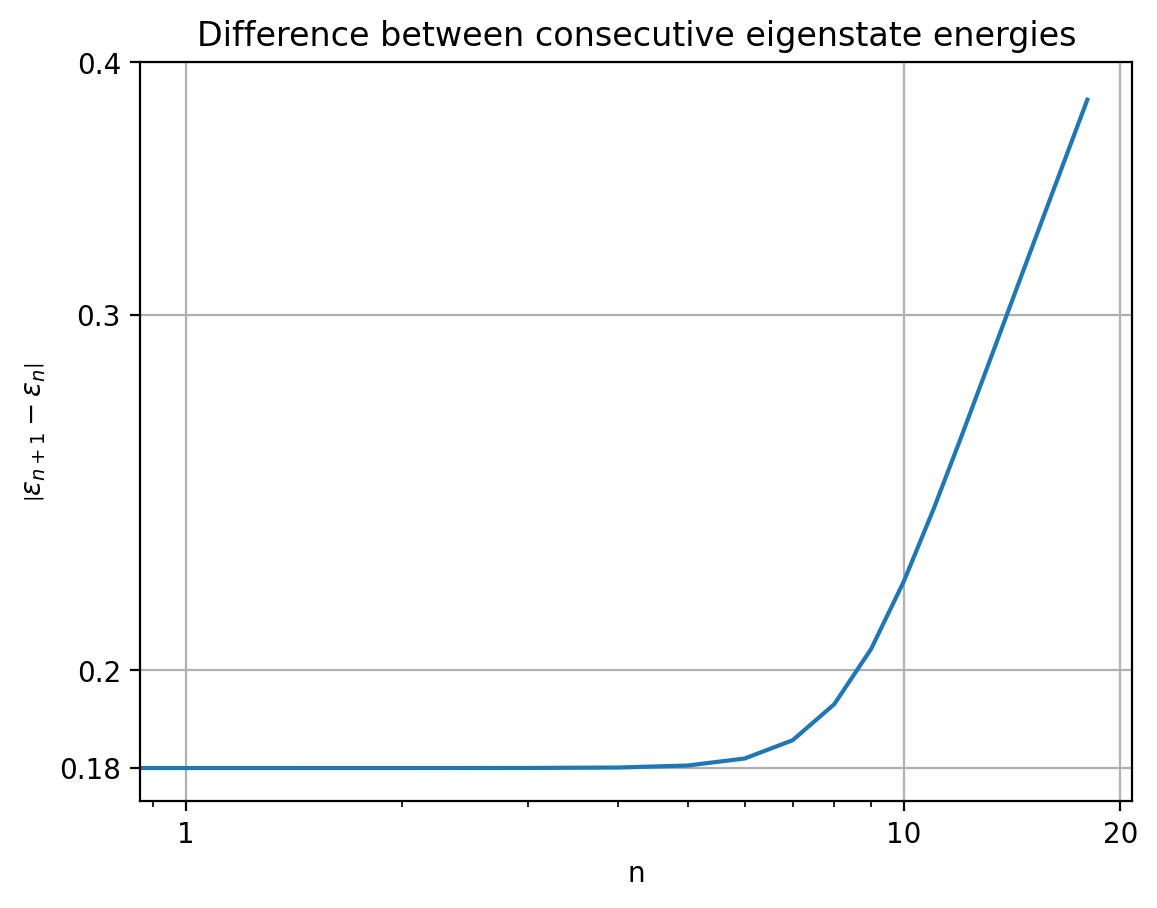
\includegraphics[width=0.7\linewidth]{diff_energies.png}
  \captionsetup{width=0.8\linewidth}
  \vspace{-.4cm}
  \caption{Differences between consecutive energies - bounded harmonic}
\end{wrapfigure}

\vspace{.5cm}

Another way of clearly observing the discrepancy, is to look at differences between
consecutive eigenstate energies calculated by the algorithm: 
For low values of $n$, the energies are evenly spaced - in accordance with the 
harmonic potential. However, for $n$ higher than around 10 the plot shifts into the
infinite well region - and produces a line with the slope of 2, as predicted by
that type of potential.

\vspace{1.3cm}

\section{Conclusion}

It is clear that numerical methods of solving the Schr{\"o}dinger
equation are indispensable in many cases. They were shown to produce
accurate solutions as well as being able to find eigenvalues of the
energy operator.

The computed eigenstate energies were shown to become more accurate
with smaller values of tolerance, up to a certain limit.
Below that limit, other sources of error were shown to be dominant,
especially for higher energies. 

The uncertainties in $x$ and $p$ were found to increase linearly
with the excitation number $n$ both in the case of the infinite well
and the bounded harmonic potential. However, only the lowest energy
state in the harmonic potential obtained the minimum possible value
corresponding to $\hbar/2$.

The limitations of approximating the harmonic potential by its 
bounded counterpart were found to become more prominent at higher
energies. There, the system appeared to behave as if the potential
was an infinite well - the eigenstate energies began to be spaced
quadratically in $n$, instead of linearly as would be the case in
the quantum harmonic oscillator.

\bibliography{refs}
\bibliographystyle{plain}

\end{document}